\documentclass[11pt, a4paper]{article}
\usepackage[utf8]{inputenc}
\usepackage[T1]{fontenc}
\usepackage[french]{babel}
\usepackage{amsmath}
\usepackage{amssymb}
\usepackage{graphicx}
\usepackage{geometry}
\usepackage{hyperref}
\usepackage{xcolor}
\usepackage{listings} % For code listings
\usepackage{pgfplots} % For heatmaps and advanced plots
\usepackage{tikz}     % For drawing with pgfplots
\pgfplotsset{compat=1.18} % Recommended for pgfplots
\usepackage{booktabs} % For professional quality tables
\usepackage{siunitx} % For typesetting numbers with units and aligning numbers in tables
\usepackage{csvsimple} % For including CSV files as tables
\usepackage{appendix} % For appendix

\geometry{a4paper, margin=2.5cm}

% Basic Python syntax highlighting
\lstdefinestyle{python}{
    language=Python,
    basicstyle=\ttfamily\small,
    literate={é}{{\'e}}1, % Handle é in listings
    keywordstyle=\color{blue},
    commentstyle=\color{green!40!black},
    stringstyle=\color{red},
    showstringspaces=false,
    breaklines=true,
    frame=single,
    numbers=left,
    numberstyle=\tiny\color{gray}
}

\title{Projet INFO-H-3000 : Planification Équitable des Tournois Round Robin avec Méta-heuristiques}
\author{Nicholas Birch de la Calle \\ Gabriel Badan \\ Milena Paques \\[1em] Enseignant : Yves De Smet \\ Assistant : Jean Rosenfeld}
\date{Mai 2025} % Updated date

\begin{document}

\maketitle

\tableofcontents
\newpage

\section{Introduction}
\subsection{Contexte}
La planification de tournois où chaque participant rencontre tous les autres une seule fois (tournoi "Round Robin" simple, ou SRR) est un problème classique en recherche opérationnelle et en gestion sportive. L'objectif de base est de s'assurer que toutes les rencontres requises aient lieu. Cependant, dans de nombreux contextes, l'équité du calendrier devient un enjeu majeur. Des avantages positionnels, comme jouer à domicile dans les sports d'équipe (football, basketball) ou jouer avec les pièces blanches aux échecs, peuvent influencer significativement l'issue des matchs et, par conséquent, le classement final du tournoi. Un calendrier qui attribue systématiquement les matchs à domicile contre les adversaires les plus faibles à une équipe, ou qui impose de longues séries de matchs à l'extérieur à une autre, peut être considéré comme injuste. Ce projet s'attaque au défi de construire des calendriers SRR qui non seulement respectent les contraintes de base, mais optimisent également l'équité selon plusieurs dimensions.

\subsection{Objectifs du Projet}
L'objectif principal de ce projet est de développer et d'évaluer des méthodes pour générer des calendriers de tournois SRR équitables pour un nombre $n$ de joueurs (supposé pair). L'équité est définie à travers un ensemble de critères quantifiables :
\begin{itemize}
    \item Équilibrage de l'avantage domicile/extérieur en fonction de la différence de force entre les adversaires (HomeStrength). Cette métrique évalue si les équipes les plus fortes ont tendance à recevoir les plus faibles, ou vice-versa.
    \item Minimisation des séries de matchs consécutifs joués à domicile ou à l'extérieur ("Pénalité de séquence").
    \item Homogénéité de la répartition des matchs domicile/extérieur entre tous les joueurs (Proxy : Max Deviation).
\end{itemize}
Pour atteindre cet objectif, nous avons exploré trois approches complémentaires :
\begin{enumerate}
    \item Une méthode exacte basée sur la Programmation Linéaire en Nombres Entiers Mixtes (MILP) pour obtenir des solutions optimales sur de petites instances.
    \item Une méta-heuristique (Recuit Simulé, SA) optimisée pour trouver des solutions de bonne qualité pour des instances de taille moyenne et grande dans un temps raisonnable.
    \item Une seconde méta-heuristique (Recherche Tabou "légère", TS) pour comparer les approches heuristiques et explorer différentes stratégies de recherche.
\end{enumerate}

\subsection{Structure du Rapport}
Ce rapport détaille la modélisation mathématique du problème (Section~\ref{sec:modelisation}), incluant la définition du problème, les variables de décision, les contraintes fondamentales et d'équité, ainsi que les métriques d'équité (HomeStrength, Pénalité de Séquence, et Max Deviation). La Section~\ref{sec:normalisation_et_objectif_sa} aborde ensuite la normalisation des métriques et la fonction objectif utilisée par la méta-heuristique. Enfin, la Section~\ref{sec:calibration_pareto_empirique} présente la méthode de calibration des poids de cette fonction objectif via l'analyse d'un front de Pareto empirique et discute de la sélection d'un point opératoire.

\section{Modélisation Mathématique}
\label{sec:modelisation}
\subsection{Définition du Problème}
Le problème consiste à générer un calendrier pour un tournoi Round Robin simple (SRR) impliquant $n$ joueurs, où $n$ est pair. Les joueurs sont numérotés de $1$ à $n$, et cet indice représente également leur classement de force (1 étant le plus fort, $n$ le plus faible). Le tournoi se déroule sur $n-1$ rondes (numérotées de $0$ à $n-2$). Dans chaque ronde, $n/2$ matchs sont joués simultanément. Chaque paire de joueurs $\{i, j\}$ doit s'affronter exactement une fois au cours du tournoi. Pour chaque match, l'un des joueurs est désigné comme jouant "à domicile" (H) et l'autre "à l'extérieur" (A). L'objectif est de produire un calendrier complet qui minimise une fonction d'équité combinant plusieurs critères.

\textbf{Entrées :}
\begin{itemize}
    \item $n$ : Le nombre de joueurs (pair).
\end{itemize}
\textbf{Sortie :}
\begin{itemize}
    \item Un calendrier complet spécifiant pour chaque ronde $r \in \{0, \dots, n-2\}$ et chaque match $(i, j)$ qui joue à domicile (avec $i, j \in \{1, \dots, n\}$).
\end{itemize}

\subsection{Variables de Décision}
\subsubsection{Variable Principale}
La décision fondamentale pour chaque match potentiel est de savoir qui joue à domicile. Nous utilisons une variable binaire principale pour cela :
\begin{equation}
    x_{i,j,r} = 
    \begin{cases} 
        1 & \text{si le joueur } i \text{ joue à domicile contre le joueur } j \text{ lors de la ronde } r \\
        0 & \text{sinon}
    \end{cases}
\end{equation}
où $P = \{1, \dots, n\}$ est l'ensemble des joueurs (avec $i \neq j$) et $R = \{0, \dots, n-2\}$ représente l'ensemble des rondes. L'indice du joueur correspond à son classement (1 étant le plus fort).

\subsubsection{Variables Auxiliaires pour l'Équité}
Pour modéliser les métriques d'équité, nous introduisons les variables auxiliaires suivantes :
\begin{itemize}
    \item $is\_home_{i,r}$: Variable binaire valant 1 si le joueur $i \in P$ joue à domicile lors de la ronde $r \in R$.
    \item $pen\_seq_{i,r}$: Variable binaire valant 1 si le joueur $i \in P$ subit une "pénalité de séquence" (deux matchs consécutifs à domicile ou à l'extérieur) entre les rondes $r$ et $r+1$. Définie pour $r \in R' = \{0, \dots, n-3\}$.
    \item $H_i$: Variable entière représentant le nombre total de matchs joués à domicile par le joueur $i \in P$.
    \item $MaxDev$: Variable continue représentant l'écart absolu maximal entre le nombre de matchs à domicile d'un joueur ($H_i$) et la moyenne idéale $\bar{H} = \frac{n-1}{2}$.
\end{itemize}

\subsection{Contraintes}
\subsubsection{Contraintes Fondamentales du Round Robin}
\begin{itemize}
    \item \textbf{Un match par joueur par ronde :} Chaque joueur doit jouer exactement un match lors de chaque ronde.
    \begin{equation}
        \sum_{j \in P, j \neq i} x_{i,j,r} + \sum_{j \in P, j \neq i} x_{j,i,r} = 1 \quad \forall i \in P, \forall r \in R
    \end{equation}
    \item \textbf{Chaque paire se rencontre une fois :} Chaque paire de joueurs $\{i, j\}$ doit s'affronter exactement une fois au cours du tournoi.
    \begin{equation}
        \sum_{r \in R} (x_{i,j,r} + x_{j,i,r}) = 1 \quad \forall i, j \in P, i < j
    \end{equation}
\end{itemize}

\subsubsection{Contraintes d'Équité}
Ces contraintes lient les variables auxiliaires aux variables de décision $x_{i,j,r}$.
\begin{itemize}
    \item \textbf{Lien $is\_home_{i,r}$ :} Détermine si un joueur est à domicile.
    \begin{equation}
        is\_home_{i,r} = \sum_{j \in P, j \neq i} x_{i,j,r} \quad \forall i \in P, \forall r \in R
    \end{equation}
    \item \textbf{Lien $pen\_seq_{i,r}$ (Pénalités Séquence) :} Une pénalité se produit si $is\_home_{i,r} = is\_home_{i,r+1}$. Ceci est linéarisé comme suit :
    \begin{align}
        pen\_seq_{i,r} &\ge is\_home_{i,r} + is\_home_{i,r+1} - 1 \quad &\forall i \in P, \forall r \in R' \\
        pen\_seq_{i,r} &\ge (1 - is\_home_{i,r}) + (1 - is\_home_{i,r+1}) - 1 \quad &\forall i \in P, \forall r \in R' 
    \end{align}
    où $R' = \{0, \dots, n-3\}$.
    \item \textbf{Lien $H_i$ (Total Domicile) :} Calcule le nombre total de matchs à domicile.
    \begin{equation}
        H_i = \sum_{r \in R} is\_home_{i,r} \quad \forall i \in P
    \end{equation}
    \item \textbf{Lien $MaxDev$ (Écart Max Domicile) :} Calcule l'écart maximal par rapport à la moyenne $\bar{H} = \frac{n-1}{2}$.
    \begin{align}
        MaxDev &\ge H_i - \bar{H} \quad &\forall i \in P \\
        MaxDev &\ge \bar{H} - H_i \quad &\forall i \in P
    \end{align}
\end{itemize}

\subsection{Métriques d'Équité}
Les objectifs d'équité sont quantifiés par les métriques suivantes, que nous cherchons à minimiser (ou, dans le cas de HomeStrength, à amener proche de zéro).

\subsubsection{HomeStrength}
Cette métrique évalue l'équilibre de la force des adversaires rencontrés par rapport au lieu du match (domicile/extérieur). Elle est définie comme la somme, sur tous les matchs, de la différence de rang entre l'adversaire et le joueur à domicile. En supposant que l'indice du joueur $k$ (de $1$ à $n$) représente son classement (1 étant le plus fort), la métrique est :
\begin{equation}
    \text{HomeStrength} = \sum_{i \in P} \sum_{j \in P, j \neq i} \sum_{r \in R} \max(0, j - i) \cdot x_{i,j,r}
    \label{eq:homestrength}
\end{equation}
où $x_{i,j,r}=1$ si le joueur $i$ (domicile) joue contre le joueur $j$ (extérieur) en ronde $r$.
Cette métrique ne somme que les différences de rang positives ($j-i > 0$), c'est-à-dire uniquement lorsque le joueur à domicile ($i$) est mieux classé que son adversaire ($j$). Une valeur élevée indique que les joueurs forts reçoivent souvent des joueurs plus faibles à domicile. L'objectif est de minimiser cette valeur pour réduire cet avantage spécifique. La normalisation de cette métrique (voir Section~\ref{subsec:normalisation_calibration}) la ramène à un intervalle $[0, 1]$.

\subsubsection{Pénalité de Séquence}
Une "pénalité de séquence" est définie comme deux matchs consécutifs joués soit à domicile (H-H), soit à l'extérieur (A-A). Le nombre total de pénalités est la somme des variables auxiliaires $pen\_seq_{i,r}$ :
\begin{equation}
    \text{TotalPenalitesSequence} = \sum_{i \in P} \sum_{r \in R'} pen\_seq_{i,r}
\end{equation}
où $R' = \{0, \dots, n-3\}$. Minimiser cette somme favorise une alternance H/A plus régulière.

\subsubsection{StdDevAdvantage (Proxy : MaxDev)}
Pour assurer une répartition homogène du nombre de matchs joués à domicile entre les joueurs, nous cherchons à minimiser la variance de $H_i$. La variance étant une fonction quadratique ($\sum (H_i - \bar{H})^2 / n$), elle ne peut être directement utilisée dans un objectif linéaire. Nous utilisons donc une approximation linéaire courante : minimiser l'écart absolu maximal par rapport à la moyenne $\bar{H} = \frac{n-1}{2}$. Cette valeur, capturée par la variable $MaxDev$, sert de proxy pour l'homogénéité de la répartition des matchs à domicile.
\begin{equation}
    \text{MaxDeviation} = MaxDev
\end{equation}

\subsection{Fonction Objectif}
\label{subsec:fonction_objectif_initiale}
Initialement, nous combinons les trois métriques d'équité principales en une fonction objectif pondérée unique. Pour HomeStrength, l'objectif est d'avoir une valeur proche de zéro. Pour les autres, c'est la minimisation.
\begin{equation}
    \text{Objectif} = f(\text{HomeStrength}, \text{TotalPenalitesSequence}, \text{MaxDeviation})
\end{equation}
La fonction exacte, incluant la pondération et la normalisation, est détaillée ci-dessous.

\subsection{Fonction Objectif Normalisée et Calibration des Poids ($\alpha, \beta$)}
\label{sec:normalisation_et_objectif_sa}
Les trois métriques d'équité -- HomeStrength (HS, Équation~\ref{eq:homestrength}), TotalPenalitesSequence (PS), et MaxDeviation (MD) -- sont de natures et d'échelles intrinsèquement différentes. Une combinaison directe dans une fonction objectif pondérée pour une méta-heuristique comme le Recuit Simulé (SA) nécessite une normalisation adéquate pour que les poids attribués à chaque critère reflètent fidèlement leur importance relative et pour que la recherche ne soit pas biaisée par les échelles disparates.

Bien qu'une normalisation basée sur des bornes théoriques (comme $S_{max}$, $D_{PS}$, $D_{MD}$ précédemment évoqués pour un modèle exact) puisse être envisagée, elle présente des inconvénients pour l'optimisation heuristique. Les maximums théoriques ne capturent souvent pas la distribution typique ou la variabilité des métriques dans l'espace des solutions exploré par une heuristique. Par exemple, une métrique pourrait avoir un maximum théorique très élevé mais varier dans une plage beaucoup plus restreinte pour la majorité des calendriers "raisonnables". Cela peut conduire à ce que certaines métriques, même après une telle normalisation, dominent l'objectif composite ou rendent l'interprétation et l'ajustement fin des poids de la fonction objectif peu intuitifs.

Pour surmonter ces limitations dans le cadre de notre méta-heuristique SA, une stratégie de \textbf{normalisation empirique} a été adoptée. Pour chaque métrique brute $M_k^{raw}$ (où $k \in \{\text{HS, PS, MD}\}$), une valeur normalisée $M_k^{emp\_norm}$ est calculée en utilisant des facteurs d'échelle dérivés de l'observation statistique des valeurs brutes de ces métriques sur un grand ensemble de calendriers divers. Spécifiquement, pour un nombre $n$ de joueurs donné, nous générons un échantillon de calendriers (par exemple, via des exécutions initiales du SA avec différents paramètres ou des constructions aléatoires) et calculons la médiane ($med_k$) et l'écart-type ($\sigma_k$) pour chaque métrique brute. La métrique normalisée empiriquement est alors définie comme :
\begin{equation}
    M_k^{emp\_norm} = \frac{M_k^{raw} - med_k}{\sigma_k} \quad \text{ou plus simplement} \quad M_k^{emp\_norm} = \frac{M_k^{raw}}{\sigma_k^{emp}}
    \label{eq:emp_norm_general}
\end{equation}
Dans notre implémentation, nous avons utilisé la seconde forme, où $\sigma_k^{emp}$ représente l'écart-type empirique (ou une mesure de dispersion similaire) servant de facteur d'échelle. Cette approche assure que les métriques normalisées se situent sur des échelles comparables qui reflètent leur variabilité typique observée en pratique, rendant la fonction objectif du SA plus équilibrée.

Le problème de la génération de calendriers équitables est ainsi traité par le SA comme un problème d'optimisation cherchant à minimiser une combinaison pondérée de ces métriques normalisées empiriquement :
\begin{equation}
    Z_{SA} = emp\_norm\_hs + \alpha \cdot emp\_norm\_ps + \beta \cdot emp\_norm\_md
    \label{eq:sa_objectif_empirique}
\end{equation}
Les paramètres $\alpha \geq 0$ et $\beta \geq 0$ représentent les poids qui modulent l'importance relative de la pénalité de séquence et de la déviation maximale par rapport à HomeStrength, toutes exprimées dans leurs échelles empiriquement normalisées. Plutôt que de fixer $\alpha$ et $\beta$ a priori, une exploration systématique de leurs valeurs est entreprise pour analyser les compromis inhérents entre les trois objectifs. Cette exploration mène à la construction d'un front de Pareto empirique, comme détaillé dans la section suivante, permettant un choix éclairé des poids.


\section{Calibration des Poids par Analyse du Front de Pareto Empirique}
\label{sec:calibration_pareto_empirique}
La calibration des poids $\alpha$ et $\beta$ de la fonction objectif du Recuit Simulé (Équation~\ref{eq:sa_objectif_empirique}) est une étape cruciale pour comprendre les compromis possibles entre les différentes dimensions de l'équité, exprimées via leurs formes normalisées empiriquement. Cette calibration a été réalisée en exécutant l'algorithme de Recuit Simulé pour un nombre $n=200$ joueurs, sur un ensemble de paires de valeurs $(\alpha, \beta)$. Typiquement, ces paires sont choisies sur une grille (par exemple, $\alpha \in [0.5, 1.5]$ et $\beta \in [0.5, 1.5]$ avec un pas de $0.1$ pour notre étude sur $n=200$).

Pour chaque calendrier résultant d'une exécution du SA avec une paire $(\alpha, \beta)$ donnée, les valeurs des trois métriques normalisées empiriquement ($emp\_norm\_hs$, $emp\_norm\_ps$, $emp\_norm\_md$) sont calculées. Ces points forment un nuage dans l'espace tridimensionnel des objectifs. À partir de cet ensemble de solutions, le front de Pareto est identifié. Un front de Pareto est constitué de l'ensemble des solutions non-dominées, c'est-à-dire des solutions pour lesquelles aucune amélioration sur un objectif n'est possible sans dégrader au moins un autre objectif.

\begin{figure}[htbp]
    \centering
    % Path updated based on workspace structure
    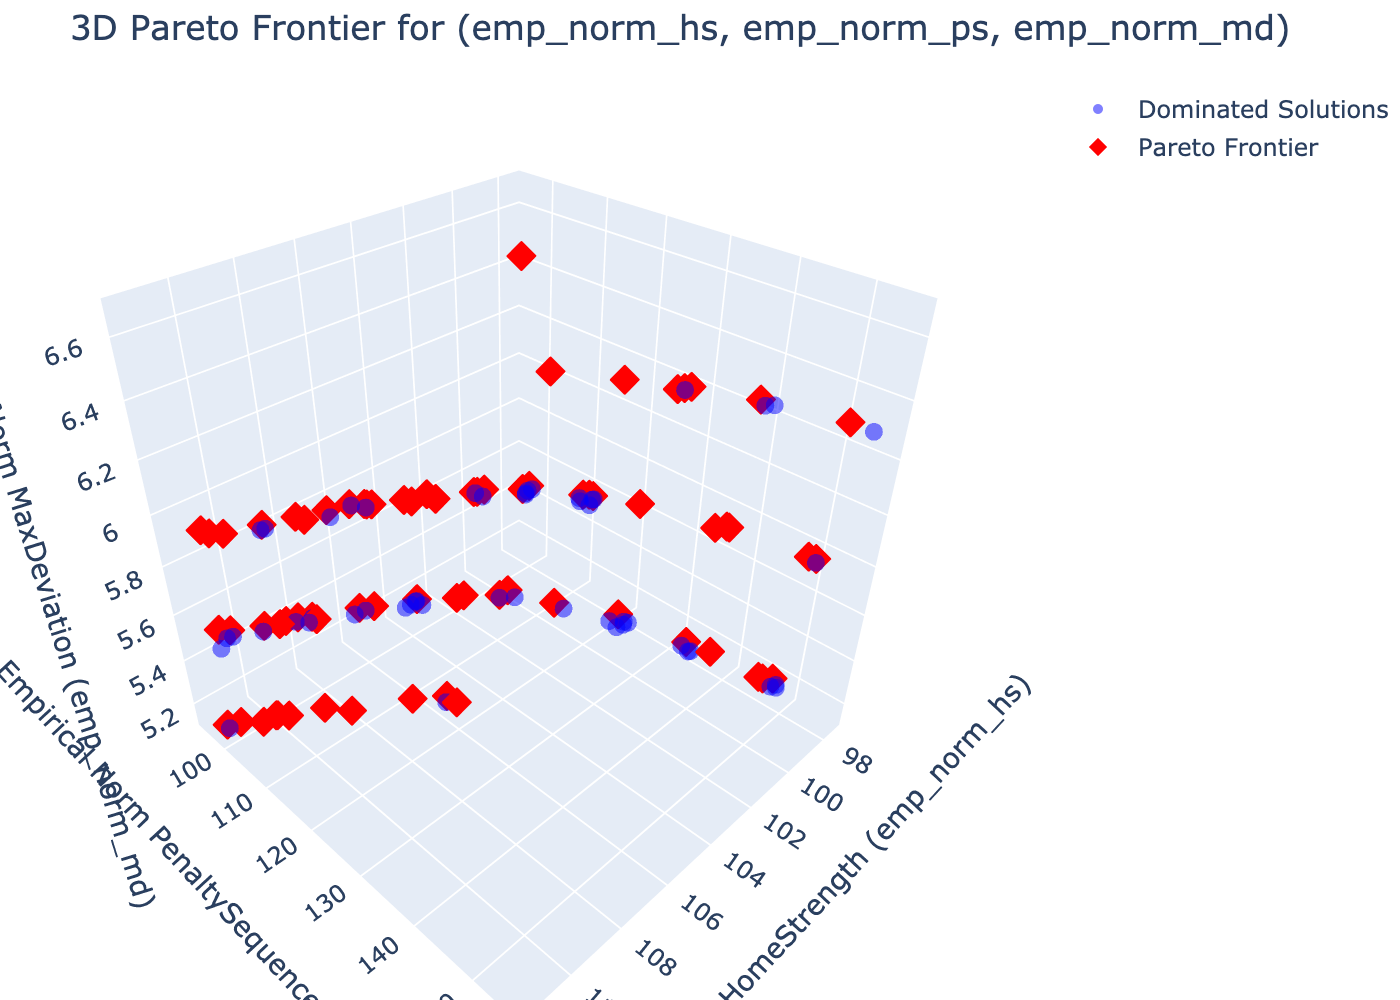
\includegraphics[width=0.9\textwidth]{../calibration_plots_n200_empirical_norm_v1/pareto_3d_static_empirical_n200.png}
    \caption{Front de Pareto 3D illustrant les compromis entre les trois métriques d'équité normalisées empiriquement ($emp\_norm\_hs$, $emp\_norm\_ps$, $emp\_norm\_md$) pour un tournoi de $n=200$ joueurs. Les points rouges représentent les solutions Pareto-optimales, tandis que les points bleus représentent les solutions dominées. Les axes représentent les valeurs des métriques normalisées empiriquement, où des valeurs plus faibles sont préférées pour chaque axe.}
    \label{fig:pareto_3d_empirique}
\end{figure}

La Figure~\ref{fig:pareto_3d_empirique} montre le front de Pareto obtenu pour $n=200$ joueurs en utilisant les métriques normalisées empiriquement. Ce front illustre visuellement les relations de compromis : par exemple, chercher à minimiser agressivement les pénalités de séquence ($emp\_norm\_ps$) pourrait conduire à une augmentation de la déviation maximale ($emp\_norm\_md$) ou à une valeur moins favorable de HomeStrength ($emp\_norm\_hs$).

Le choix d'une solution spécifique (et donc d'une paire $(\alpha, \beta)$) sur le front de Pareto dépend des priorités de l'organisateur du tournoi. La métrique HomeStrength (Équation~\ref{eq:homestrength}), même normalisée empiriquement, mesure toujours la tendance des joueurs les mieux classés à affronter à domicile des joueurs moins bien classés. Une valeur élevée de $emp\_norm\_hs$ est donc généralement considérée comme inéquitable car elle confère un avantage potentiellement systématique aux équipes déjà fortes. Par conséquent, une stratégie de sélection judicieuse pourrait privilégier les points sur le front qui offrent une faible valeur pour $emp\_norm\_hs$, tout en maintenant des niveaux acceptables pour $emp\_norm\_ps$ et $emp\_norm\_md$. Il est important de noter que, en raison de la nature de la normalisation empirique (division par $\sigma_k^{emp}$), les valeurs numériques des $emp\_norm$ ne sont pas directement interprétables comme des pourcentages ou des rapports à un maximum théorique, mais servent à comparer les solutions entre elles sur une base équitable.

Pour notre étude avec $n=200$, l'analyse du front de Pareto a mis en évidence plusieurs combinaisons $(\alpha, \beta)$ intéressantes. La configuration avec $\alpha=0.50$ et $\beta=1.50$ a généré une solution caractérisée par les valeurs suivantes pour les métriques normalisées empiriquement : $emp\_norm\_hs \approx 99.16$, $emp\_norm\_ps \approx 153.60$, et $emp\_norm\_md \approx 5.90$. Cette solution est considérée comme un compromis équilibré. Bien que la valeur de $emp\_norm\_ps$ soit plus élevée que pour d'autres points sur le front, ce choix reflète une priorisation de la métrique $emp\_norm\_hs$, qui est significativement plus basse avec cette configuration. La minimisation de HomeStrength est cruciale car cette métrique reflète un aspect fondamental de l'équité sportive : éviter que les équipes fortes bénéficient indûment d'un calendrier favorable en termes d'avantage du terrain contre des adversaires plus faibles. Ce point offre donc un bon équilibre entre la réduction de cet avantage positionnel (faible $emp\_norm\_hs$) et le maintien des autres critères d'équité ($emp\_norm\_ps$ et $emp\_norm\_md$) à des niveaux acceptables dans le contexte des compromis identifiés par le front de Pareto.

En conclusion, l'exploration systématique de l'espace des poids $(\alpha, \beta)$ et l'analyse du front de Pareto empirique fournissent un outil décisionnel robuste. Elles permettent de choisir un calendrier qui correspond au mieux aux préférences spécifiques en matière d'équité, en se basant sur la performance relative des solutions dans l'espace des objectifs normalisés empiriquement.

\end{document}
